%%%%%%%%%%%%%%%%%%%%%%%%%%%%%%%%%%%%%%%%%%%%%%%%%%%%%%%%%%%%%%%%%%
%%%%%%%% ICML 2010 EXAMPLE LATEX SUBMISSION FILE %%%%%%%%%%%%%%%%%
%%%%%%%%%%%%%%%%%%%%%%%%%%%%%%%%%%%%%%%%%%%%%%%%%%%%%%%%%%%%%%%%%%

% Use the following line _only_ if you're still using LaTeX 2.09.
%\documentstyle[icml2010,epsf,natbib]{article}
% If you rely on Latex2e packages, like most moden people use this:
\documentclass{article}

% For figures
\usepackage{graphicx} % more modern
%\usepackage{epsfig} % less modern
\usepackage{subfigure} 

% For citations
\usepackage{natbib}

% For algorithms
\usepackage{algorithm}
\usepackage{algorithmic}

\usepackage{tikz}
% \usepackage{tikz-qtree,tikz-qtree-compat}
\usetikzlibrary{arrows,shapes,positioning,fit,shapes.misc,matrix,decorations.text,shapes.geometric,trees}


% As of 2010, we use the hyperref package to produce hyperlinks in the
% resulting PDF.  If this breaks your system, please commend out the
% following usepackage line and replace \usepackage{icml2010} with
% \usepackage[nohyperref]{icml2010} above.
\usepackage{hyperref}

% Packages hyperref and algorithmic misbehave sometimes.  We can fix
% this with the following command.
\newcommand{\theHalgorithm}{\arabic{algorithm}}

% Employ the following version of the ``usepackage'' statement for
% submitting the draft version of the paper for review.  This will set
% the note in the first column to ``Under review.  Do not distribute.''
% \usepackage{icml2010} 
% Employ this version of the ``usepackage'' statement after the paper has
% been accepted, when creating the final version.  This will set the
% note in the first column to ``Appearing in''
\usepackage[accepted]{icml2010}


% The \icmltitle you define below is probably too long as a header.
% Therefore, a short form for the running title is supplied here:
\icmltitlerunning{Submission and Formatting Instructions for ICML 2010}

\begin{document} 

\twocolumn[
\icmltitle{Hierarchical Aspect-Sentiment Analysis for Online Reviews
           (using Deep Learning Techniques?)}

% It is OKAY to include author information, even for blind
% submissions: the style file will automatically remove it for you
% unless you've provided the [accepted] option to the icml2010
% package.
\icmlauthor{Arzoo Katiyar}{ak979@cornell.edu}
\icmladdress{Cornell University}

% You may provide any keywords that you 
% find helpful for describing your paper; these are used to populate 
% the "keywords" metadata in the PDF but will not be shown in the document
\icmlkeywords{multi-aspect sentiment analysis, deep learning}

\vskip 0.3in
]

% \begin{abstract} 
% ICML 2010 full paper submissions are due February 1, 2010. Reviewing will
% be blind to the identities of the authors, and therefore identifying
% information should not appear in any way in papers submitted for
% review. Submissions must be in PDF, 8 page length limit.
% \end{abstract} 

\section{Progress made}
% \section{Motivation}
\label{submission}
\subsection{Proposed Model}
Let $R$ denote a review for a product $P$ and let \{$s_{1}$, $s_{2}$, $\dots$ $s_{n}$\} are the sentences in a review such that every sentence has an associated aspect. For simplicity, we assume that there is a single aspect associated with every sentence. Let \{$a_{1}$, $a_{2}$ $\dots$ $a_{k}$\} be the aspects that can be arranged in a hierarchy. Again for the sake of simplicity, we consider a very simple hierarchy as shown below. 
\begin{center}
\begin{tikzpicture}  [scale=1.2,transform shape]
\tikzset{frontier/.style ={distance from root=12pt}}
% \tikzstyle{level 1}=[sibling distance=52mm] 
% \tikzstyle{level 2}=[sibling distance=18mm] 
    \node {$P$}
    child {node {$a_{1}$}}
    child {node {$a_{2}$}}
    child {node {$\dots$}}
    child {node {$a_{k}$}};
\end{tikzpicture}
\end{center}
Since every sentence has an aspect, we can modify the above diagram to include the sentences as below. 
\begin{center}
\begin{tikzpicture}  [scale=1.2,transform shape]
\tikzset{frontier/.style ={distance from root=12pt}}
% \tikzstyle{level 1}=[sibling distance=52mm] 
% \tikzstyle{level 2}=[sibling distance=18mm] 
    \node {$P$}
    child {node {$a_{1}$}
	  child {node {$s_{1}$}}
	  child {node {$s_{2}$}}}
    child {node {$a_{2}$}
	  child {node {$s_{3}$}}}
    child {node {$\dots$}}
    child {node {$a_{k}$}
	  child {node {$\dots$}}
	  child {node {$s_{n}$}}};
\end{tikzpicture}
\end{center}
Trivially we know that a review need not contain sentences corresponding to every aspect for that product. Also \emph {we assume that we know a gold standard hierarchy for the product} we consider. \\
In order to use the model described in \cite{Socher}, we want to find vector representation of the sentences at the leaf level in the hierarchy. 
\subsection{Sentence Model}
We want to compute a vector for a sentence $s$ given the sequence of words in $s$ and a vector for each of the words. We propose to use hierarchical convolutional neural network similar to described in \cite{ Kalchbrenner}. At the initial stage of composition, the value of a feature in the sentence vector is a function of the values of the same feature in the word vectors. In the next stage, we take compositionality to yield local effects and then yield increasingly more global effects across all the words in the sentence by adopting convolutional kernels of gradually increasing sizes that ultimately span the whole sentence. Figure 1 shows the hierarchical convolutional neural network for sentential compositionality where the bottom layer represents a single feature across all the word vectors in the sentence and the top layer is the value of corresponding feature in the resulting sentence vector. 

\begin{figure}[ht]
\vskip 0.2in
\begin{center}
\centerline{\includegraphics[width=\columnwidth]{cnn.jpg}}
\caption{Figure used from \cite{Kim} to show the part of tree structure for the LAPTOP review corpus.}
\label{icml-historical}
\end{center}
\vskip -0.2in
\end{figure} 



User generated online reviews contain rich information related to the various aspects of a product. A recent study \cite{Chen} shows that the customers seek opinions from other users by reading their reviews for the product. Due to the recent popularity of these sites, large number of reviews for different products are available thus leading to the need to extract and evaluate opinions and present them to the user. 

Most of the previous work deal with finding the overall sentiment of a review or recently on multi-aspect sentence labeling where each sentence in a review is labeled according to the aspect it discusses along-with finding aspect-specific star ratings for each review. An example review from OpenTable.com as provided in the paper \cite{Lu} to illustrate the aspects of a review for a restaurant is :

`` The food was very good, but it took over half an hour to be seated, ... and the service was terrible. The room was very noisy and cold wind blew in from a curtain next to our table. Desserts were very good, but because of [the] poor service, I'm not sure we'll ever go back$!$ " 

The above review expresses positive opinion toward the restaurant's food but negative opinion towards the ambiance and the service. The goal was to label each sentence in the review with the aspect it expresses (food, ambiance, service) and also find the sentiment for every aspect. A more recent work \cite{Kim} introduces a hierarchical structure in sentiment analysis for reviews. If we consider the example in Figure 1 from the paper, it describes a tree structure over the different aspects of the reviews. Each node in the tree is itself a two-level tree, where the root represent the aspect and the children represent the associated sentiment polarities. Different users are interested in different levels of granularity of aspects and sentiments. Some users may be interested in general aspects such as screen or CPUs in a laptop, while other users might be interested in more specific aspects such as CPU frequency or cache size. Thus it is desirable to have a hierarchy of the different aspects(at each granular 
level). The paper infer the aspect-sentiment tree from the review texts.

Another independent work on sentiment analysis \cite{Socher} introduces a Recursive Neural Tensor Network(RNTN) for sentiment composition. Semantic word spaces for single words have lately been used by many researchers. Since these vector spaces do not capture the meaning of the longer phrases properly, compositionality in semantic vector spaces has received a lot of attention by the researchers. This paper uses fine-grained sentiment labels for phrases in the parse tree of the sentences and use RNTN for sentiment composition for the positive/negative sentiment classification in a sentence. 

The general idea of this project is to find out if the deep learning techniques introduced above can be used to find the overall sentiment of a document using some similar compositionality techniques over the sentences (or phrases$?$). However, we restrict ourselves to the online user-generated product reviews where there is a possibility of finding a structure in the document and our goal is to be able to use this hierarchy similar to the parse tree in the case of recursive neural networks.

\begin{figure}[ht]
\vskip 0.2in
\begin{center}
\centerline{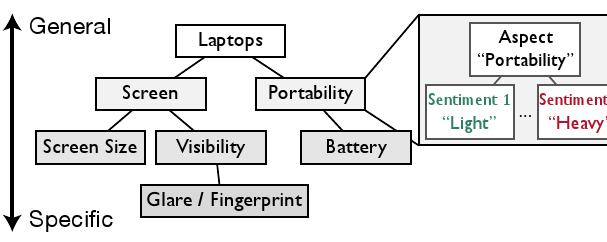
\includegraphics[width=\columnwidth]{fig.jpeg}}
\caption{Figure used from \cite{Kim} to show the part of tree structure for the LAPTOP review corpus.}
\label{icml-historical}
\end{center}
\vskip -0.2in
\end{figure} 


\section{Statement of the Problem}
Given an online product review $R$ = \{$sen_{1}$, $sen_{2}$, ..\} we want to find out the sentiment polarities \{$p_{a_{1}}$, $p_{a_{2}}$, ..\}  for the different aspects \{$a_{1}$, $a_{2}$, ..\} at various granular level \{$g_{1}$, $g_{2}$, ..\} and thus find out the sentiment($S$) of the overall product review. 

As a starting point, we want to assume that the hierarchy among the different aspects of the products is already provided and hence the goal is to be able to come up with an equivalent vector representation of the sentences (phrases or words $?$) under the aspects at the finest granularity level. The immediate key challenges in this project involve 
\begin{itemize}
 \item Finding out the semantic vector representation for sentences under an aspect in the hierarchy.\\
 We may need to consider using vector representations for the words or phrases instead of the sentences.
 \item Compositionality of the sentiments in the sentences under an aspect in the hierarchy. \\
 However, this does not seem intuitive for the case where a single aspect is discussed at different places in the review. If all the sentences about a particular aspect are next to each other, then we expect that the sentences are related to each other in some way through discourse analysis.
 \item Compositionality of the sentiments over the finer aspects to find the sentiment of the parent aspect.\\
 Since the hierarchical structure need not be a binary tree, we need to figure out how (if) the compositionality as described in the paper \cite{Socher} need to be modified.
\end{itemize}

\section{General Approach}
As discussed above, we would like to assume that the hierarchy among the different aspects of the product is already known. Then, we would like to formulate the problem similar to the semantic compositionality over a sentence. We start with the parsing of the product review based on the hierarchical structure. Then assign initial uniformly distributed vector representations to the sentences and use the same compositionality function as described in the paper cited above. Similarly, we want to find out if using the words or phrases from the sentences is better able to capture the sentiments for an aspect.

The first and foremost task is to be able to find out if our problem is captured well by the model we propose. Since there has not been much work on finding the sentiment of the review using the sentiments of the different aspects in the review, we are restricted to the hierarchy model in the paper cited above for the initial experiments.

Another interesting idea from the paper that builds aspects-hierarchy for online reviews is to find out how it performs on any document (any text). It will be interesting to find out the different clusters within a document that it might generate. 

\section{Resources}
We hope to conduct experiments on two publicly available datasets, Amazon.com reviews of laptops (LAPTOPS) and digital SLRs available at http://uilab.kaist.ac.kr/research/WSDM11 The readings are provided in the references section. 

\section{Schedule}
\begin{itemize}
 \item {\bf 16 March} : Start with some initial experiments based on the model that we finalise before this period.
 \item {\bf 20 April} : Provide the results from the experiments on the datasets and compare the results with the existing techniques.
 \item {\bf 12 May} : Improve the model with the suggestions, if any, during the presentation and also finish the report writing by then.
\end{itemize}


\bibliography{example_paper}
\bibliographystyle{icml2010}

\end{document} 


% This document was modified from the file originally made available by
% Pat Langley and Andrea Danyluk for ICML-2K. This 2010 version was
% created by Thorsten Joachims & Johannes Fuernkranz, 
% slightly modified from the 2009 version by Kiri Wagstaff and 
% Sam Roweis's 2008 version, which is slightly modified from 
% Prasad Tadepalli's 2007 version which is a lightly 
% changed version of the previous year's version by Andrew Moore, 
% which was in turn edited from those of Kristian Kersting and 
% Codrina Lauth. Alex Smola contributed to the algorithmic style files.  


